%%%%%%%% ICML 2018 EXAMPLE LATEX SUBMISSION FILE %%%%%%%%%%%%%%%%%

\documentclass{article}

% Recommended, but optional, packages for figures and better typesetting:
\usepackage{microtype}
\usepackage{graphicx}
\usepackage{subfigure}
\usepackage{booktabs} % for professional tables

% Added by wenlong lyu
\usepackage{amsmath}
\usepackage[plain]{fancyref}
\usepackage{bm}
\usepackage{todonotes}
\usepackage{placeins}

% hyperref makes hyperlinks in the resulting PDF.
% If your build breaks (sometimes temporarily if a hyperlink spans a page)
% please comment out the following usepackage line and replace
% \usepackage{icml2018} with \usepackage[nohyperref]{icml2018} above.
\usepackage{hyperref}

% Attempt to make hyperref and algorithmic work together better:
\newcommand{\theHalgorithm}{\arabic{algorithm}}

% Use the following line for the initial blind version submitted for review:
\usepackage{icml2018}

% If accepted, instead use the following line for the camera-ready submission:
%\usepackage[accepted]{icml2018}

% The \icmltitle you define below is probably too long as a header.
% Therefore, a short form for the running title is supplied here:
\icmltitlerunning{Batched Bayesian Optimization via Multi-objective Acquisition Ensemble for Automated Analog Circuit Design}

\begin{document}

\twocolumn[
\icmltitle{Batched Bayesian Optimization via Multi-objective Acquisition Ensemble for Automated Analog Circuit Design}

% It is OKAY to include author information, even for blind
% submissions: the style file will automatically remove it for you
% unless you've provided the [accepted] option to the icml2018
% package.

% List of affiliations: The first argument should be a (short)
% identifier you will use later to specify author affiliations
% Academic affiliations should list Department, University, City, Region, Country
% Industry affiliations should list Company, City, Region, Country

% You can specify symbols, otherwise they are numbered in order.
% Ideally, you should not use this facility. Affiliations will be numbered
% in order of appearance and this is the preferred way.
\icmlsetsymbol{equal}{*}

\begin{icmlauthorlist}
\icmlauthor{Aeiau Zzzz}{equal,to}
\icmlauthor{Bauiu C.~Yyyy}{equal,to,goo}
\icmlauthor{Cieua Vvvvv}{goo}
\icmlauthor{Iaesut Saoeu}{ed}
\icmlauthor{Fiuea Rrrr}{to}
\icmlauthor{Tateu H.~Yasehe}{ed,to,goo}
\icmlauthor{Aaoeu Iasoh}{goo}
\icmlauthor{Buiui Eueu}{ed}
\icmlauthor{Aeuia Zzzz}{ed}
\icmlauthor{Bieea C.~Yyyy}{to,goo}
\icmlauthor{Teoau Xxxx}{ed}
\icmlauthor{Eee Pppp}{ed}
\end{icmlauthorlist}

\icmlaffiliation{to}{Department of Computation, University of Torontoland, Torontoland, Canada}
\icmlaffiliation{goo}{Googol ShallowMind, New London, Michigan, USA}
\icmlaffiliation{ed}{School of Computation, University of Edenborrow, Edenborrow, United Kingdom}

\icmlcorrespondingauthor{Cieua Vvvvv}{c.vvvvv@googol.com}
\icmlcorrespondingauthor{Eee Pppp}{ep@eden.co.uk}

% You may provide any keywords that you
% find helpful for describing your paper; these are used to populate
% the "keywords" metadata in the PDF but will not be shown in the document
\icmlkeywords{Bayesian Optimization, Automated analog circuit design}

\vskip 0.3in
]

% this must go after the closing bracket ] following \twocolumn[ ...

% This command actually creates the footnote in the first column
% listing the affiliations and the copyright notice.
% The command takes one argument, which is text to display at the start of the footnote.
% The \icmlEqualContribution command is standard text for equal contribution.
% Remove it (just {}) if you do not need this facility.

%\printAffiliationsAndNotice{}  % leave blank if no need to mention equal contribution
\printAffiliationsAndNotice{\icmlEqualContribution} % otherwise use the standard text.


\begin{abstract}
    Bayesian optimization methods are promising for the optimization of black-box functions that are expensive to evaluate. In this paper, a novel batch Bayesian optimization approach is proposed. The parallelization is realized via a multi-objective ensemble of multiple
    acquisition functions. In each iteration, the multi-objective optimization of the multiple acquisition functions is performed to search for
    the Pareto front of the acquisition functions. The batch of inputs are then selected from the Pareto front. The Pareto front represents the best trade-off between the multiple acquisition functions. Such a policy for batch Bayesian optimization can significantly improve the efficiency of optimization. The proposed method is compared with several
    state-of-the-art batch Bayesian optimization algorithms using analytical
    benchmark functions and real-world analog integrated circuits. The experimental
    results show that the proposed method is competitive compared with the
    state-of-the-art algorithms.
\end{abstract}

\section{Introduction}

% % TODO: more introduction to the importance of anlog IC sizing, as the reviewers may not have much knowledge of circuit design
%
The advancement of modern society is driven by the development of Integrated
Circuits (IC). Unlike the digital circuits where the design flow is already
highly automated, the automation of analog circuit design is still a
challenging problem.

Traditionally, the design parameters of analog circuits like widths and lengths of
transistors are manually calculated by designers with their experience and the
understanding of the design specifications. However, due to the progress of IC
manufacture technology forecasted by Moore's law, the circuit devices become
more and more complicated, and the parasitic effect of the circuits can no
longer be ignored. On the other hand, the demands for high-performance,
low-power analog circuits are increasing. It is much more difficult to
meet the performance and time-to-market requirements with manual circuit design.
Automated analog circuit design has thus attracted much research interest in
the past decade~\cite{rutenbar2007hierarchical}.

% TODO: Traditional methods using offline model and simulated based methods are
% not good
The analog circuit design automation problems can be formulated as optimization
problems. The aim is to find the optimal design parameters that provide the
best circuit performance, which can be represented by a figure of merit (FOM)
scalar real-valued function. Prior works about analog circuit optimization
include offline model-based approaches
~\cite{colleran2003optimization,daems2003simulation,wang2014enabling} and
simulation-based approaches. The offline model-based methods try to build
global models of the FOM via manual calculation or regression with simulated
data and then optimize the cheap-to-evaluate models. The problem with this
approach is that the accurate models are usually hard to get. For example,
in~\cite{wang2014enabling}, 100,000 randomly simulated points are used to train
a sparse polynomial model for an amplifier circuit with ten design parameters.

Simulation-based methods, instead, treat the performances of the circuits as black-box functions. The performances are obtained from circuit simulations. Global optimization
algorithms are directly applied to the black-box functions. For
simulation-based circuit optimization methods, meta-heuristic
algorithms~\cite{phelps2000anaconda, liu2009analog} are widely used. Although
these algorithms can explore the whole design space, they have relatively low
convergence rate. When the circuit simulation takes a long time, both
model-based and simulation-based approaches can be very time-consuming.

% TODO: Bayesian optimization is a sequential algorithm, there is a need to
% parallelize it

In recent years, the Gaussian process (GP)~\cite{GPML} model has been
introduced for the automated design of analog circuits to reduce the
required number of circuit simulations. In~\cite{liu2014gaspad}, GP is combined
with differential evolution algorithm. Recently, the Bayesian optimization
(BO)~\cite{shahriari2016taking} algorithm has also been applied for analog
circuit optimization. In~\cite{lyu2017efficient}, the Bayesian optimization
algorithm is firstly introduced for the single- and multi-objective
optimization of general analog circuits and has shown to be more efficient
compared with other simulation-based approaches. In~\cite{wang2017efficient},
the Bayesian optimization algorithm is combined with adaptive Monte-Carlo
sampling to optimize the yield of analog circuits and static random-access
memory (SRAM).

The Bayesian optimization algorithm is a well-studied algorithm and has
demonstrated to be promising for the automated design of analog circuits.
However, the standard Bayesian optimization algorithm is sequential, it chooses
only one point at each iteration by optimizing the acquisition function. It is
often desirable to select a batch of points at each iteration, the sequential
property of Bayesian optimization limits its further applications in multi-core computer systems.

The Bayesian optimization algorithm has been extended to enable batch
selection. Some prior works, like the qEI \cite{qEI}, qKG \cite{wu2016parallel}
and parallel predictive entropy search (PPES)~\cite{shah2015parallel}
approaches, consider to search for the optimal batch selection for a given
acquisition function. These methods usually involve some approximations or
Monte-Carlo sampling, and thus scales poorly as the batch size increases. Other
works, including the simulation matching (SM)~\cite{azimi2010batch} method, the
batch-UCB (BUCB, BLCB for minimization
problems)~\cite{desautels2014parallelizing} method, the parallel UCB with pure
exploration (GP-UCB-PE)~\cite{contal2013parallel} method, and the local
penalization (LP)~\cite{gonzalez2016batch} method, adopted the \emph{greedy}
strategies that select individual points until the batch is filled.

% TODO: Beiefly introduce my algorithm
All the batch Bayesian optimization algorithms mentioned above choose to use single acquisition function.
And except for the SM method~\cite{azimi2010batch} and LP method~\cite{gonzalez2016batch} which can use arbitrary acquisition
function, other parallelization methods rely on a specific acquisition
function. The UCB acquisition function must be used for BUCB and GP-UCB-PE, and
the knowledge gradient (KG) acquisition function must be used for the qKG algorithm. As is stated
in~\cite{hoffman2011portfolio}, no single acquisition function can always
outperform other acquisition functions. Relying on one acquisition function may
result in poor performance.

In this paper, we propose to parallelize the Bayesian optimization algorithm
via the Multi-objective ACquisition Ensemble (MACE). The proposed MACE method
exploits the disagreement between different acquisition functions to enable
batch selection. At each iteration, after the GP model is updated, multiple
acquisition functions are selected. We then perform multi-objective
optimization to find the \emph{Pareto front} (PF) of the acquisition functions.
The PF represents the best trade-off between these acquisition functions. When
batch evaluations are possible, we can sample multiple points on the PF to accelerate the optimization.

The MACE algorithm is tested using several analytical benchmark functions and
two real-world analog circuits, including an operational amplifier with ten
design parameters and a class-E power amplifier with twelve design parameters.
The BLCB method~\cite{desautels2014parallelizing}, local penalization method with expected improvement
acquisition function (EI-LP)~\cite{gonzalez2016batch}, qEI \cite{qEI} methods and qKG \cite{wu2016parallel} are compared with
MACE. The proposed MACE method achieved competitive performance when compared
with the state-of-the-art algorithms listed in the paper.

\section{Background}

% TODO: See how other people describe GP and BO}

\subsection{Problem Formulation}

% TODO: The circuit performance comes from \bf{circuit} simulation}
% TODO: format, citation of HSPICE/spectre}
% TODO: See how other analog circuit optimization paper formulate the problem}

We handle the scenarios where topology of the analog circuit is fixed, this is
practical as thare are usually a lot of classical topologies for given design
task. Once the circuit topology is fixed, the designer has to choose the
appropriate design parameters according to the specifications and the circuit
device model. What we want to do is to automatically search for the optimal
design parameters, the problem can then be formulated as a bound-constrained
black-box optimization problem:

\begin{equation}
    \label{eq:Formulation}
    \text{minimize}~\mathrm{FOM}(\bm{x})
\end{equation}

where $\bm{x} \in \textrm{D} \subset \textrm{R}^d$ is the design variables
and $f_i(\bm{x})$ represents the $i$-th cared circuit performance like gain
or phase margin of an amplifier. and the $\mathrm{FOM}(\bm{x})$ is the
design objective. Given the design parameters $\bm{x}$, the FOM value can be
obtained via circuit simulation using softwares like HSPICE or spectre.

% TODO: Explain the noise

\subsection{Gaussian Process Regression}

We model the $\mathrm{FOM}(\bm{x})$ in \eqref{eq:Formulation} with Gaussian
process (GP) model~\cite{GPML}. The GP model is the most commonly used model
for Bayesian optimization, the advantage of GP is that it can give a
well-calibrated uncertainty of prediction. GP is characterized by a mean
function $m(\bm{x})$ and a covariance function $k(\bm{x}, \bm{x'})$. In this
paper, we use squared-exponential ARD kernel, and a constant mean function
$m(\bm{x}) = \mu_0$ for all our experiments.

Given a new data point $\bm{x}$, the prediction of $f(\bm{x})$ is
not a scalar value, but a predictive distribution 
\begin{equation}
f(\bm{x}) \sim N(\mu(\bm{x}),
\sigma^2(\bm{x}))
\label{eq:GPRPred}
\end{equation}
where $\mu(\bm{x})$ and $\sigma^2(\bm{x})$ can be expressed as
\begin{equation}
        \begin{array}{lll}
            \mu(\bm{x}) &=& \mu_0 + k(\bm{x},X)K^{-1}(\bm{y} - \mu_0) \\
            \sigma^2(\bm{x}) &=& \sigma_f^2 - k(\bm{x}, X)K^{-1}k(X, \bm{x})
        \end{array}
    \label{eq:GPRPredEqNoisy}
\end{equation}
where $k(\bm{x}, X) = (k(\bm{x}, \bm{x}_1), \dots, k(\bm{x},
\bm{x}_N))^T$ and $k(X, \bm{x}) = k(\bm{x}, X)^T$. The
$\mu(\bm{x})$ can be viewed as the prediction of the function value, while
the $\sigma^2(\bm{x})$ is a measure of uncertainty. 

\subsection{Bayesian Optimization}

Bayesian optimization~\cite{shahriari2016taking} was proposed for the
optimization of expensive black-box functions. It consists of two essential
ingredients, i.e., the probabilistic surrogate models and an acquisition
function. The probabilistic surrogate models provide the prediction with
uncertainties. They are refined incrementally with newly observed data.
Acquisition function is used to explore the state space based on the surrogate
model optimally. The procedure of Bayesian optimization is described in
Algorithm~\ref{alg:BayesianOptAlgo}.

\begin{algorithm}
\caption{Bayesian Optimization}
\label{alg:BayesianOptAlgo}
\begin{algorithmic}[1]
\STATE Initial Sampling
\STATE Construct initial GP model
\FOR{t = 1, 2, \dots}
\STATE Construct the acquisition function
\STATE Find $\bm{x}_t$ that optimizes the acquisition function
\STATE Sample $y_t = f(\bm{x}_t)$
\STATE Update probabilistic surrogate model
\ENDFOR
\STATE Return best $f(\bm{x})$ recorded during iterations
\end{algorithmic}
\end{algorithm}

In Bayesian optimization described in Algorithm~\ref{alg:BayesianOptAlgo}, the acquisition function is used to balance the exploration and exploitation during the optimization. The acquisition function considers both the predictive value and the uncertainty. There are a lot of existing acquisition functions, examples include the lower confidence bound (LCB), the probability of improvement (PI), and the expected improvement (EI).

The LCB function is defined as follows:
\begin{equation}
    \label{eq:LCB}
    \mathrm{LCB}(\bm{x}) = \mu(\bm{x}) - \kappa \sigma(\bm{x})
\end{equation}
Where the $\mu(\bm{x})$ and the $\sigma(\bm{x})$ are the predictive value and uncertainty of GP. $\kappa$ is a parameter that balances the exploitation and exploration. 

Following the suggestion of~\cite{brochu2010tutorial}, the $\kappa$ in \eqref{eq:LCB} is defined as:
\begin{equation}
    \label{eq:LCB}
    \begin{array}{lll}
        \kappa &=& \sqrt{\nu \tau_t} \\
        \tau_t &=& 2 \log(t^{d/2+2} \pi^2 / 3 \delta)
    \end{array}
\end{equation}
Where $t$ is the number of current iteration. $\nu$ and $\delta$ are two user defined parameters, we fix $\nu = 0.5$ and $\delta = 0.05$ in this paper for the proposed MACE algorithm and our implementation of the BLCB algorithm.

The PI and EI function are defined as
\begin{equation}
    \label{eq:PI_EI}
    \begin{array}{lll}
        \mathrm{PI}(\bm{x}) &=& \Phi(\lambda) \\
        \mathrm{EI}(\bm{x}) &=& \sigma(\bm{x}) (\lambda \Phi(\lambda) + \phi(\lambda))     \\
        \mathrm{\lambda}    &=& \displaystyle \frac{\tau - \xi - \mu(\bm{x})}{\sigma(\bm{x})}, 
    \end{array}
\end{equation}
where $\tau$ is the current best value objective value, and $\xi$ is a small positive jitter to improvement the ability of exploration. The $\Phi(.)$ and $\phi(.)$ functions are the CDF and PDF functions of normal distribution.

% TODO: discuss the different behaviours of LCB, EI, PI

There are also other acquisition function, like the knowledge gradient~\cite{scott2011correlated} function, predictive entropy search~\cite{hernandez2014predictive}. A portforlio of several acquisition functions is also possible~\cite{hoffman2011portfolio}.

\section{Proposed Batched Bayesian Optimization Algorithm}

\subsection{Multi-objective Optimization of Acquisition Functions}\label{sec:MOForumlation}

\textcolor{red}{See how other MOBO paper formulate multi-objective optimization}

\textcolor{red}{ALERT: COPIED FROM MY TCAS-I paper}

Multi-objective optimization~\cite{MO_overview} can be formulated as:
\begin{equation}
    \label{eq:MOFormulation}
    \begin{aligned}
        & \text{minimize} & & f_1(\bm{x}),~\dots~,f_m(\bm{x})
    \end{aligned}
\end{equation}

For multi-objective optimization, there are more than one objecive to optimize, and usually there does not exist a single solution that simultaneously optimize all these objectives. A design $\bm{x}_1$ is said to be \emph{dominate} by $\bm{x}_2$ if $\forall i \in \{1\dots m\},~f_i(\bm{x}_1) \le f_i(\bm{x}_2)$ and $\exists j \in \{1\dots m\}, f_j(\bm{x}_1) < f_j(\bm{x}_2)$. A design is \emph{Pareto-optimal} if it is not dominated by any other point and dominate at least one point. The whole set of the non-dominated points in the design space is called the \emph{Pareto set}, and the set of non-dominated points in the objective space is called the \emph{Pareto front}. It is often unlikely to get the whole Pareto front as there might be infinite points on the front, the goal of multi-objective optimization is to find a set of designs that approximates the true Pareto front.

There exist many mature multi-objective optimization algorithms, like the non-dominated sorting based genetic algorithm (NSGA-II)~\cite{nsgaii}, and the multi-objective evolutionary algorithm based on decomposition (MOEA/D)~\cite{moead}. In this paper, the multi-objective optimization based on differential evolution (DEMO)~\cite{demo} is used to solve multi-objective optimization problems.


% When we have more than one objective to optimize, the problem is formulated as:

\subsection{MACE}

We propose a novel heuristic for the parallelization of Bayesian optimization.
The parallelization is realized via multi-objective ensemble of multiple
acquisition functions. When we have multiple acquisition functions built from
the same GP model, they may not disagree with each other about which point is
most promising, for example, the value of LCB function always decreases as the
$\sigma(\bm{x})$ increases, however, for the PI function, when $\sigma{\bm{x}}$
increases, the value of PI would decrease when $\mu(\bm{x}) < \tau$, and
increase when $\mu(\bm{x}) > \tau$.

% TODO: discuss the difference of acquisition functions: LCB: do not avoid repeated sampling, EI: always positive

With multi-objective optimization, the disagreement between different
acquisition function can be used for the parallelization of Bayesian
optimization. In the standard Bayesian optimization, one acquisition function
is specified, and in each iteration, the single-objective optimization is
performed to optimize the acquisition function; in our proposed MACE algorithm,
multiple acquisition function is pre-specified by the user, in each iteration,
the DEMO multi-objective optimization algorithm is applied to find the Pareto
front of the acquisition functions. Once the Pareto front is obtained, we can
then sample from the Pareto front, and then evaluate these sampled points in
parallel.

% TODO: We illustrate the proposed MACE algorithm using the Branin-Hoo function~\cite{dixon1978global}
% TODO: plot contour of Branin/Ei/LCB/PI, plot the PS and the PF

We select the LCB, EI and PI acquisition function in our implementation of the MACE algorithm, but other acquisition functions like KG and PES can also be incorporated into the MACE framework. The proposed MACE algorithm is described in Algorithm~\ref{alg:MACE}.

\begin{algorithm}
\caption{Multi-objective Acquisition Ensemble Algorithm}
\label{alg:MACE}
\begin{algorithmic}[1]
\STATE Initial Sampling
\STATE Construct initial GP model
\FOR{t = 1, 2, \dots}
    \STATE Construct the LCB, EI and PI function according to \eqref{eq:LCB} and \eqref{eq:PI_EI}
    \STATE Find the Pareto front of LCB, EI, PI function using the DEMO algorithm
    \STATE Randomly sample B points $\bm{x}_1, \dots, \bm{x}_B$ from the Pareto front
    \STATE Evaluate $\bm{x}_1, \dots, \bm{x}_B$ to get $y_1 = f(\bm{x}_1),~\dots~,y_B = f(\bm{x}_B)$
    \STATE Update the GP model
\ENDFOR
\STATE Return best $f(\bm{x})$ recorded during iterations
\end{algorithmic}
\end{algorithm}

\section{Experimental Results}

The proposed MACE algorithm was tested using eight benchmark functions and two
real-world analog circuits. Four state-of-the-art parallel Bayesian optimization
methods were compared, including the BLCB
algorithm~\cite{desautels2014parallelizing}, the local penalization method with
EI acquisition function (EI-LP)~\cite{gonzalez2016batch}, the qEI and qKG
methods~\cite{qEI,wu2016parallel}\footnote{We implemented the BLCB algorithm as
the available open source implementations only allow discrete input. For the
EI-LP method, the code is downloaded from
https://github.com/SheffieldML/GPyOpt. The code for qEI and qKG is downloaded
from https://github.com/wujian16/Cornell-MOE}.

For the MACE, BLCB, and EI-LP method, the ARD squared-exponential kernel is
used and the GP models are fitted by maximum likelihood estimations (MLE); for
the qKG and qEI methods, the ARD Matern52 kernels are used, and the GP
hyperparameters are integrated via MCMC sampling. The Matern52 kernel and MCMC
integration are the default strategies of the qKG and qEI implementations and
it is unclear in the documentation about how to change the GP settings.

\begin{table}[!htb]
    \centering
    \caption{Summary of the analytical benchmark functions}
    \label{tab:summaryanalygical}
    \begin{tabular}{llllllll}
        \toprule
         Function           & Dimension        & Search domain             \\ \midrule
         Branin             & 2                & $[-5,  10]\times[0, 15]$  \\
         Alpine1            & 5                & $[-10, 10]^5$             \\
         Hartmann6          & 6                & $[0,   1]^6$              \\
         Eggholder          & 2                & $[-512, 512]^2$           \\
         Ackley2            & 2                & $[-32, 32]^2$             \\
         Ackley10           & 10               & $[-32, 32]^{10}$          \\
         Rosenbrock2        & 2                & $[-5,  10]^2$             \\
         Rosenbrock10       & 10               & $[-20, 20]^{10}$          \\
        \bottomrule
    \end{tabular}
\end{table}

\begin{table*}[!htb]
    \centering
    \caption{Optimization results of the benchmark functions}
    \label{tab:result_analytical}
    \begin{tabular}{lllllllllll}
        \toprule
                & Eggholder                &  Branin              &  Alpine1              & Hartmann6                   \\ \midrule
        MACE-1  & 87.65$\pm$75.83          &  1.05e-5$\pm$1.31e-5          & 2.66305$\pm$1.05844            & 0.0646869$\pm$0.0621189 \\
        LCB-1   & 153.9$\pm$112.8          &  6.86e-5$\pm$1.13e-4          & 5.66812$\pm$1.76973            & 0.125565$\pm$0.122684   \\
        EI-1    & 172.8$\pm$132.2          &  1.62e-2$\pm$1.63e-2          & 2.46061$\pm$1.56079            & 0.110561$\pm$0.146809   \\
        MACE-4  & 46.38$\pm$40.89          &  \textbf{4.62e-6$\pm$6.64e-6} & \textbf{0.903805$\pm$0.835209} & \textbf{0.0275738$\pm$0.052254}  \\
        BLCB-4  & 56.86$\pm$35.91          &  4.32e-5$\pm$6.33e-5          & 1.8843$\pm$0.938873            & 0.06447$\pm$0.0621176   \\
        EI-LP-4 & \textbf{44.68$\pm$56.45} &  2.11e-2$\pm$1.84e-2          & 1.0059$\pm$0.456865            & 0.0540446$\pm$0.0558557 \\
        qKG-4   & 106.4$\pm$67.64          &  2.65e-1$\pm$2.70e-1          & 3.01513$\pm$1.13414            & 0.47134$\pm$0.18939     \\
        qEI-4   & 72.13$\pm$52.08          &  3.29e-4$\pm$1.14e-3          & 2.7074$\pm$1.05145             & 0.186088$\pm$0.116323   \\
        \hline
                & Ackley2                       &  Rosenbrock2               & Ackley10              & Rosenbrock10        \\ \midrule
        MACE-1  & 1.71474$\pm$1.12154           &  0.026173$\pm$0.051189              & 3.1348$\pm$0.447874           & 499.697$\pm$300.899 \\
        LCB-1   & 1.624$\pm$0.926437            &  0.0201124$\pm$0.0205367            & 3.14797$\pm$0.519164          & 517.944$\pm$288.955 \\
        EI-1    & 1.0136$\pm$0.985858           &  13.5508$\pm$9.52734                & 18.8006$\pm$0.652136          & 1367.08$\pm$637.507 \\
        MACE-4  & 1.07906$\pm$0.886466          &  \textbf{0.00095416$\pm$0.00093729} & \textbf{2.56439$\pm$0.535488} & \textbf{158.116$\pm$50.0024} \\
        BLCB-4  & 1.40051$\pm$1.02849           &  0.00191986$\pm$0.00180895          & 3.27543$\pm$0.735501          & 406.819$\pm$127.351 \\
        EI-LP-4 & \textbf{0.284265$\pm$0.24634} &  2.73645$\pm$2.05923                & 18.2682$\pm$0.608564          & 721.351$\pm$327.365 \\
        qKG-4   & 5.59394$\pm$1.80595           &  5.03976$\pm$3.72014                & 18.197$\pm$0.764103           & 705.112$\pm$412.762 \\
        qEI-4   & 2.87373$\pm$1.02405           &  10.1881$\pm$15.0432                & 18.3686$\pm$0.501869          & 655.208$\pm$340.954 \\
        \bottomrule
    \end{tabular}
\end{table*}


\subsection{Benchmark Problems}

We tested the MACE algorithm and other parallel BO methods using eight commonly used benchmark
functions, as summarized in Table~\ref{tab:summaryanalygical}.


For all functions except the two 10D functions, we set the number of initial
random sampling to $N_{init} = 20$ and the number of iterations to $N_{iter} =
45$. Batch size is set to $B = 4$, the total number of function evaluations is
$N_{init} + B \times N_{iter}$. For the 10D Ackley and 10D Rosenbrock functions, we set
$N_{init} = 100$ and $N_{iter} = 175$. The experiments were repeated ten
times to average the random fluctuations.

We also ran the MACE algorithm in sequential mode and compared with the EI and LCB
acquisition functions. The sequential EI and LCB based Bayesian optimization
are implemented by setting the batch size $B = 1$ for EI-LP and BLCB
respectively.


The mean convergence plots of the tested algorithms on the benchmark functions are
given in Figure~\ref{fig:CovPlotBenchmark}, the statistics of the final
optimization results are listed in Table~\ref{tab:result_analytical}. As can be
seen in Figure~\ref{fig:CovPlotBenchmark} and Table~\ref{tab:result_analytical}, when running in sequential mode, the MACE
algorithm is competitive with the LCB and EI acquisition functions. The sequential MACE (MACE-1)
algorithm gave better performances than the sequential EI (EI-1) and sequential LCB (LCB-1) algorithms in the Eggholder,
Branin, Hartmann6, Ackley10, and Rosenbrock10 functions. Also, the parallel
MACE (MACE-4) gave the best performances among all the tested algorithms for
six out of the eight benchmark functions, and has shown dramatic speedup
compared to the sequential MACE.


% when running with batch size $B = 4$, the
% MACE algorithm gives the best performance for six out of the eight benchmarks.
% For the 2D Ackley function, EI-LP is the best algorithm, while for the
% Eggholder function, the MACE, BLCB, and EI-LP have quite similar performance.
% Compare the batch MACE and the sequential MACE, the speedup is also dramatic.

\subsection{Operational Amplifier}

%TODO: Introduce the importance of OpAmp and PA

The operational amplifier~\cite{wang2014enabling} shown in
Figure~\ref{fig:schDAC2014} is used to test the Bayesian optimization algorithms. The circuit is designed
using the 180nm process. It has 10 design parameters, including the lengths
and widths of transistors, the resistance of the resistors and the capacitance of the
capacitors. The circuit is simulated using the commercial HSPICE circuit simulator.

\begin{figure}[!htb]
    \begin{center}
        \centerline{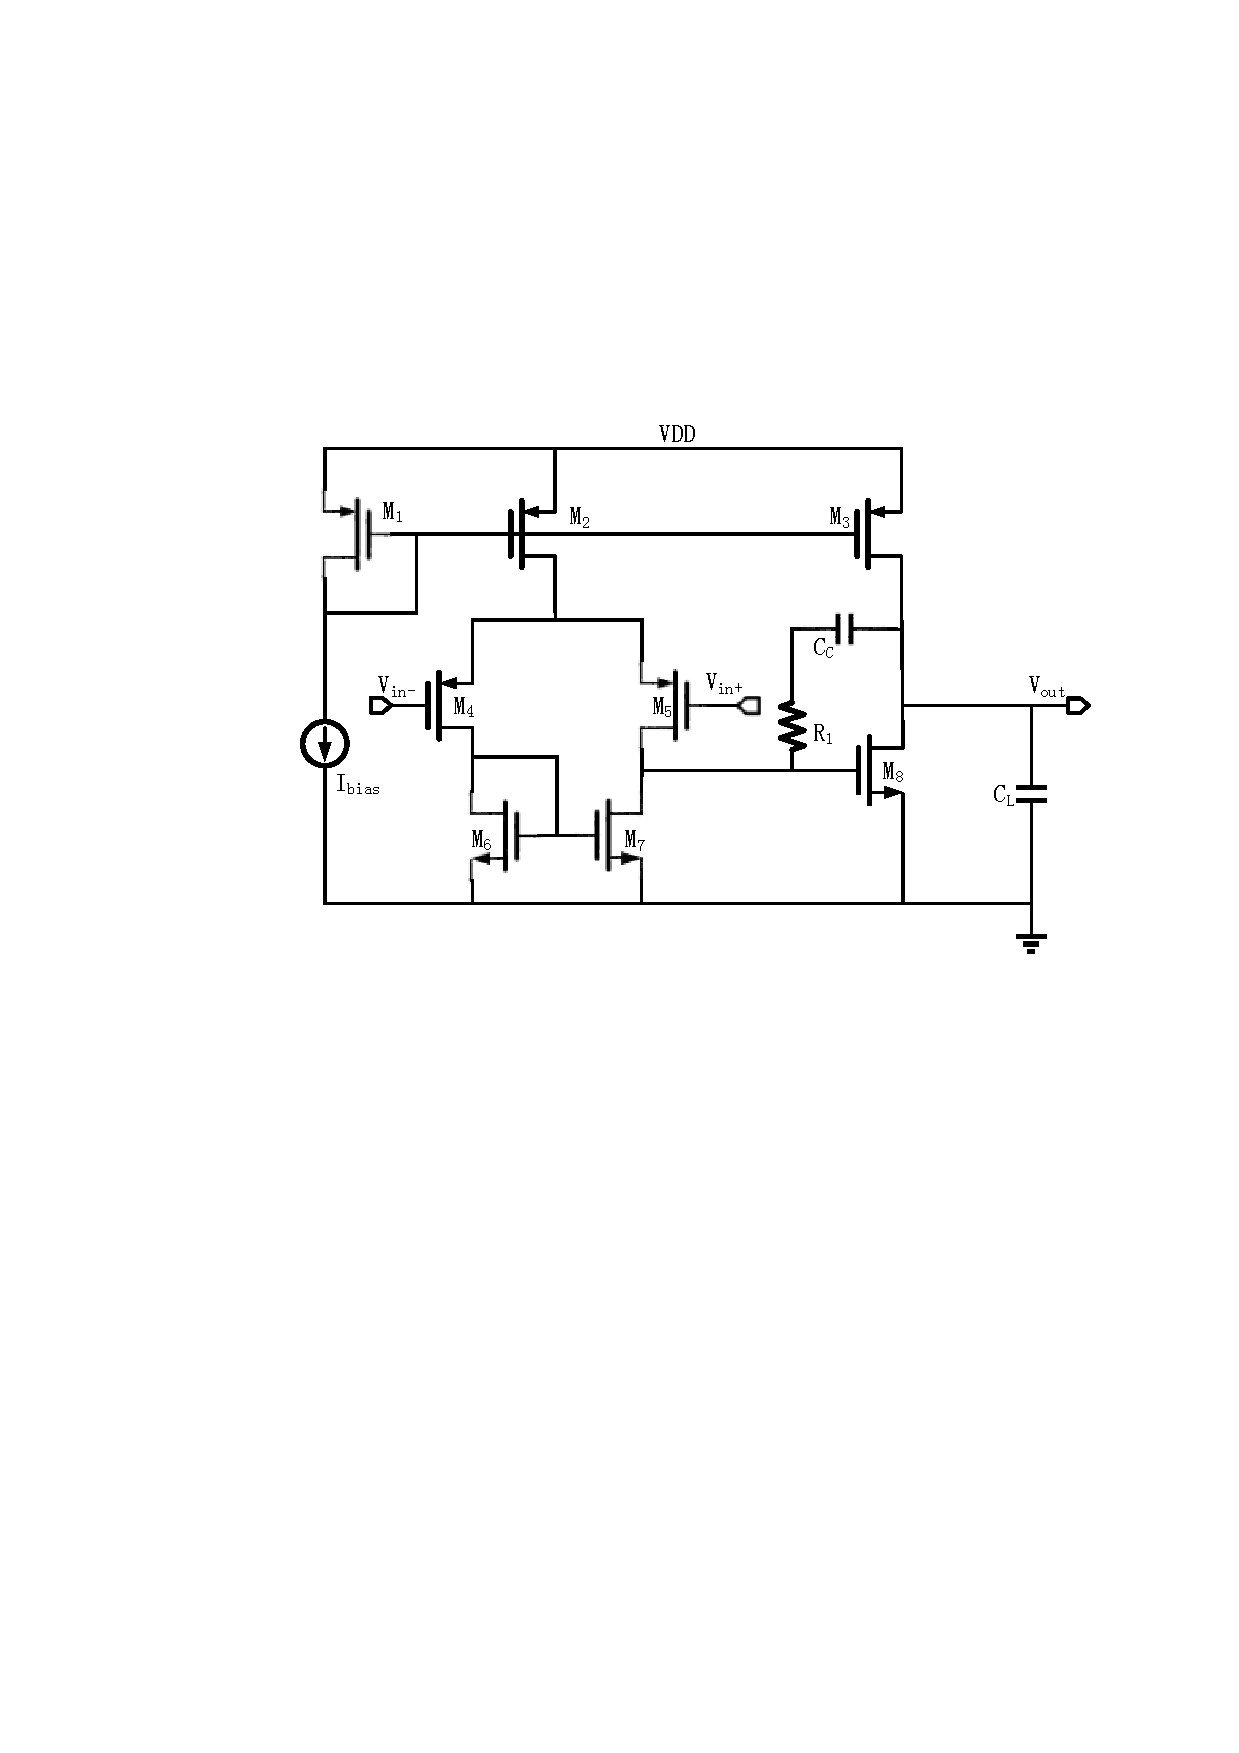
\includegraphics[width=\columnwidth]{./img/sopam.pdf}}
        \caption{Schematic of the operational amplifier}
        \label{fig:schDAC2014}
    \end{center}
    \vskip -0.2in
\end{figure}

We want to maximize the gain, unit gain frequency (UGF) and the phase margin (PM) for this amplifier. The Figure of Merit $FOM$ is constructed as
$$
\mathit{FOM} = -1.2 \times \mathit{gain} - 10 \times \mathit{UGF} - 1.6 \times \mathit{PM}.
$$

For this circuit, we compared the MACE algorithm with the BLCB and EI-LP
algorithms. The qKG and qEI are not compared as the computation of qEI and qKG
acquisition functions become very slow for the ten-dimensional functions.

\begin{figure}[!htb]
\vskip 0.2in
\begin{center}
\centerline{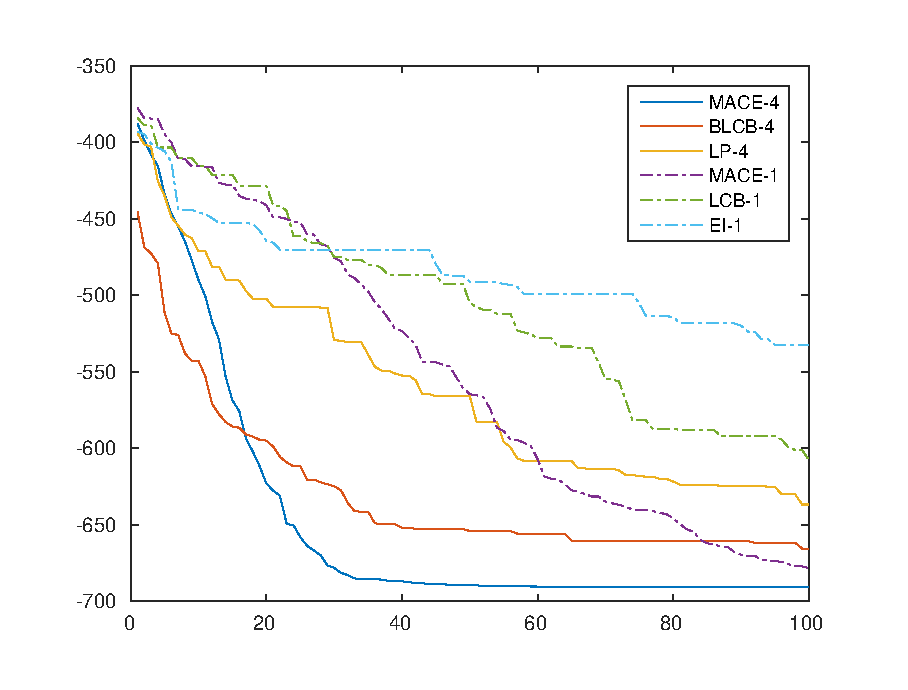
\includegraphics[width=\columnwidth]{./img/mean_DAC2014.eps}}
\caption{Optimization results of the operational amplifier}
\label{fig:resDAC2014}
\end{center}
\vskip -0.2in
\end{figure}


We run the algorithms in sequential mode and batch mode. For the batch mode,
the batch size is set to $B = 4$. The number of initial random sampling is set to
$N_{init} = 100$, and the number of iterations is set to $N_{iter} = 100$.


\begin{table}[!htb]
    \centering
    \caption{Optimization results of the operational amplifier}
    \label{tab:result_opamp}
    \begin{tabular}{llll}
        \toprule
        Algorithm & Results     \\ \midrule
        MACE-1    & -678.174$\pm$21.7445 \\
        LCB-1     & -607.583$\pm$51.9786 \\
        EI-1      & -532.555$\pm$66.942  \\
        MACE-4    & \textbf{-690.3$\pm$0.104963}  \\
        BLCB-4    & -665.442$\pm$23.066  \\
        EI-LP-4   & -636.675$\pm$35.7359 \\
        \bottomrule
    \end{tabular}
\end{table}


The mean convergence plot for the sequential and batch runs are given in
Figure~\ref{fig:resDAC2014}. The mean and standard deviation of the final
optimized FOM values are listed in Table~\ref{tab:result_opamp}. As can be
seen, on average, the batch MACE algorithm had the fastest convergence rate
compared with the sequential MACE algorithm and other parallel algorithms. It
should also be noted that the final optimized FOM values given by MACE-4 have
very small deviation (0.105) compared with other algorithms.

% The mean convergence plot for the sequential and batch runs are shown in
% Figure~\ref{fig:resDAC2014}. As can be seen, the MACE algorithm gave better
% solution compared with other algorithms, the sequential MACE algorithm found
% better solution than BLCB and EI-LP with batch size $B = 4$, which showed that
% the multi-objective acquisition ensemble is more robust than relying on single
% acquisition function; compared with the sequential MACE algorithm, the MACE
% algorithm with batch size $B = 4$ showed considerable speedup.


\begin{figure}[!htb]
    \begin{center}
        \centerline{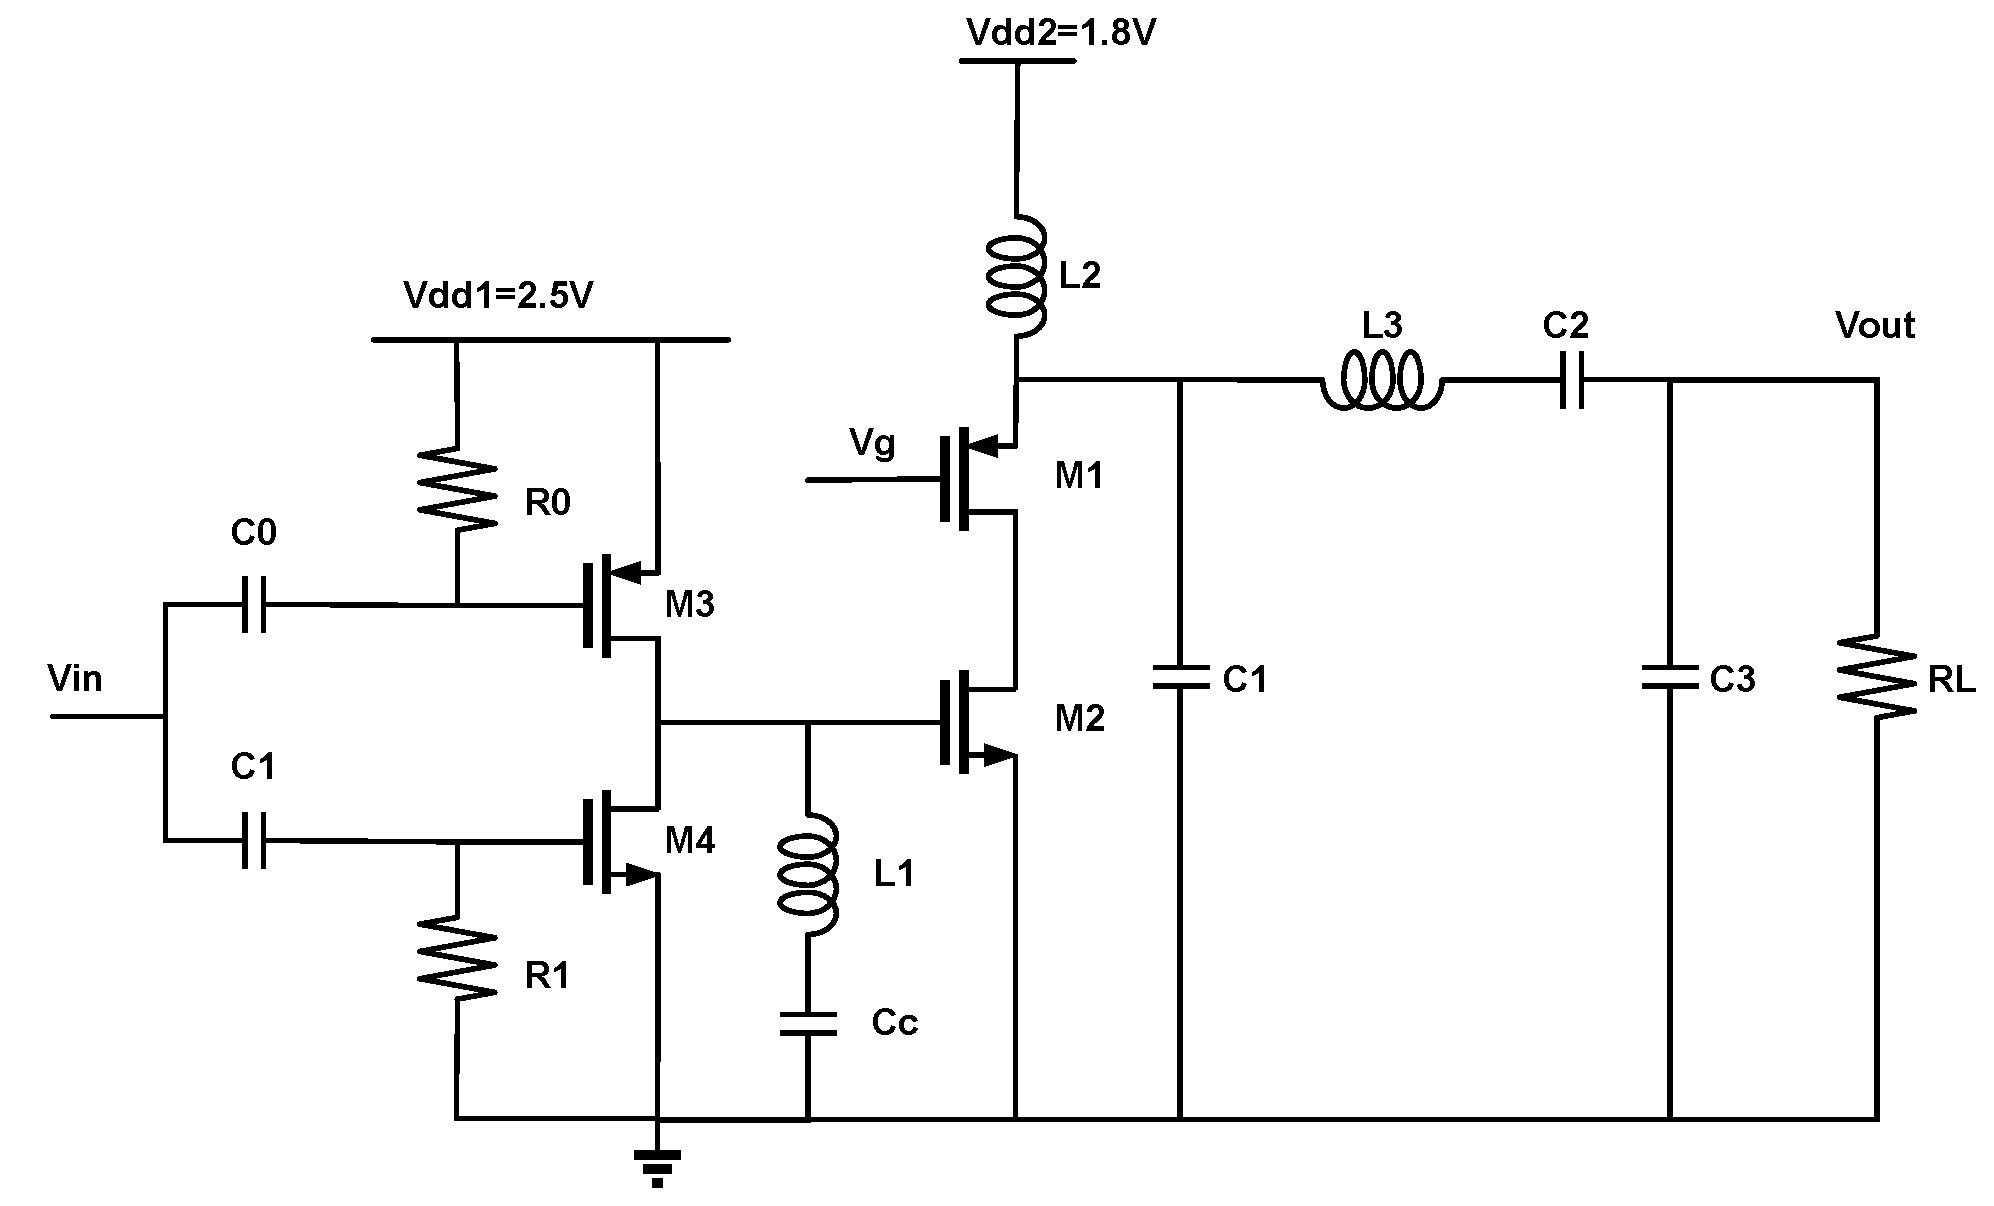
\includegraphics[width=\columnwidth]{./img/classE.eps}}
        \caption{Schematic of the power amplifier}
        \label{fig:schPA}
    \end{center}
    \vskip -0.15in
\end{figure}

\subsection{Class-E Power Amplifier}


The class-E power amplifier shown in Figure~\ref{fig:schPA} is used to test the Bayesian optimization algorithms. The
circuit is designed using the 180nm process with 12 design parameters, the
circuit is simulated by the commercial HSPICE circuit simulator to get its performances.



For this power amplifier, we aim to maximize the power added efficiency (PAE) and the output power (Pout), the Figure of Merit $FOM$ is constructed as
$$
\mathit{FOM} = -3 \times \mathit{PAE} - \mathit{Pout}.
$$

The MACE, BLCB, and EI-LP algorithms were tested in both sequential and batch
modes. The number of initial sampling is $N_{init} = 100$. The number of
iterations is $N_{iter} = 100$. The batch size is set to $B = 4$. The total
number of HSPICE simulations is 500 for each batch run and 200 for each
sequential run.

\begin{figure}[!htb]
    \begin{center}
        \centerline{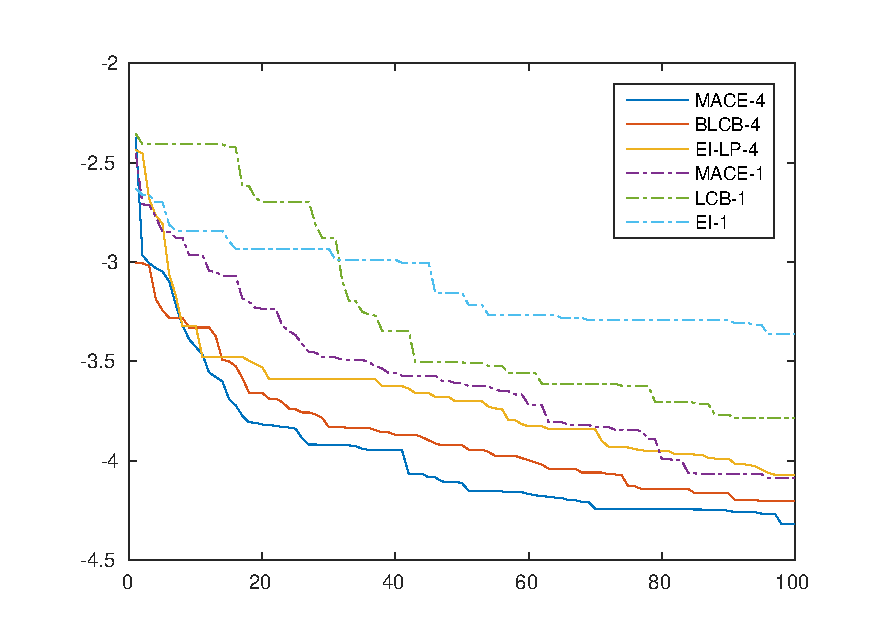
\includegraphics[width=\columnwidth]{./img/ClassE_mean.eps}}
        \caption{Optimization results of the class-E power amplifier}
        \label{fig:resClassE}
    \end{center}
    \vskip -0.2in
\end{figure}


The optimization results of the class-E power amplifier are given in
Figure~\ref{fig:resClassE} and Table~\ref{tab:result_PA}. We can see that the
MACE outperformed the BLCB and EI-LP in both sequential and batch mode. For the
batch runs, the MACE converges fastest among the three algorithms, while the
sequential MACE (MACE-1) has comparable performance as the batch EI-LP
(EI-LP-4) method.

\begin{table}[!htb]
    \centering
    \caption{Optimization results of the power amplifier}
    \vskip 0.15in
    \label{tab:result_PA}
    \begin{tabular}{llll}
        \toprule
        Algorithm & Results               \\ \midrule
        MACE-1    & -4.08608$\pm$0.296647 \\
        LCB-1     & -3.78533$\pm$0.335532 \\
        EI-1      & -3.36407$\pm$0.307489 \\
        MACE-4    & \textbf{-4.31762$\pm$0.347026} \\
        BLCB-4    & -4.20266$\pm$0.211102 \\
        EI-LP-4   & -4.07233$\pm$0.244436 \\
        \bottomrule
    \end{tabular}
    \vskip -0.1in
\end{table}

\section{Conclusion}

In this paper, a batched Bayesian optimization algorithm is proposed for the
automation of analog circuit design. the parallelization is achieved via
multi-objective ensemble of acquisition function. In each iteration, the
candidate points are sampled from the Pareto front of multiple acquisition
functions. We compared the proposed MACE algorithm using analytical benchmark
functions and real-world circuits, it is shown that the MACE algorithm is
competitive compared with state-of-the-art method listed in the paper.


\FloatBarrier

%%%%%%%%%%%%%%%%%%%%%%%%%%%%%%%%%%%%%%%%%%%%%%%%%%%%%%%%%%%%%%%%%%%%%%%%%%%%%%%
%%%%%%%%%%%%%%%%%%%%%%%%%%%%%%%%%%%%%%%%%%%%%%%%%%%%%%%%%%%%%%%%%%%%%%%%%%%%%%%

\bibliography{ref}
\bibliographystyle{icml2018}


\end{document}


% This document was modified from the file originally made available by
% Pat Langley and Andrea Danyluk for ICML-2K. This version was created
% by Iain Murray in 2018. It was modified from a version from Dan Roy in
% 2017, which was based on a version from Lise Getoor and Tobias
% Scheffer, which was slightly modified from the 2010 version by
% Thorsten Joachims & Johannes Fuernkranz, slightly modified from the
% 2009 version by Kiri Wagstaff and Sam Roweis's 2008 version, which is
% slightly modified from Prasad Tadepalli's 2007 version which is a
% lightly changed version of the previous year's version by Andrew
% Moore, which was in turn edited from those of Kristian Kersting and
% Codrina Lauth. Alex Smola contributed to the algorithmic style files.
